% ======================================================================
% METODOLOGIA - Enhanced LaTeX with Figures and Tables (Version 2)
% ======================================================================
% Required packages:
% \usepackage{graphicx}
% \usepackage{booktabs}
% \usepackage{csvsimple}
% \usepackage{caption}
% \usepackage{subcaption}

\section{Metodologia}
\label{sec:metodologia}

Aquest treball proposa una metodologia estructurada en cinc capes: anàlisi exploratòria, modelització ML (Lasso, Gradient Boosting, EBM), estratègia \emph{filter-then-interact} amb EBM en tres fases, explicabilitat per a RCA, i validació/industrialització. L'arquitectura garanteix rendiment predictiu i interpretabilitat alineada amb el domini farmacèutic.

\subsection{Capa d'anàlisi exploratòria}
\label{subsec:capa_analisi_exploratoria}

Activitats d'exploració i comprensió del conjunt de dades:

\begin{enumerate}
    \item \textbf{Anàlisi de la distribució de variables:} Estudi de la distribució de la variable objectiu (qualitat de la proteïna) i de les variables predictores.
    \item \textbf{Detecció de valors atípics:} Identificació de dades anòmales que poden afectar el rendiment dels models.
    \item \textbf{Anàlisi de correlacions:} Estudi de les relacions lineals entre variables per detectar redundàncies i possibles col·linealitats.
    \item \textbf{Reducció de dimensionalitat basada en correlació:} Eliminació de variables altament correlacionades per simplificar el model i evitar multicolinealitat.
    \item \textbf{Anàlisi de qualitat de les dades:} Avaluació de la completesa i consistència de les dades, així com la identificació de valors faltants.
\end{enumerate}

\subsection{Capa de modelització de ML}
\label{subsec:capa_modelitzacio_ml}

Es van avaluar tres famílies de models per establir una línia base:

\begin{enumerate}
    \item \textbf{Lasso (Least Absolute Shrinkage and Selection Operator):} Model lineal amb regularització L1 que realitza selecció de característiques de manera automàtica. Aquest model serveix com a línia base i proporciona una primera aproximació a les variables més rellevants.

    \item \textbf{Gradient Boosting (XGBoost/LightGBM):} Models d'ensemble basats en arbres de decisió que capturen relacions no lineals complexes. Aquests models ofereixen alt rendiment predictiu però són menys interpretables.

    \item \textbf{Explainable Boosting Machine (EBM):} Model additiu generalitzat (GAM) basat en boosting que manté la interpretabilitat mentre captura efectes no lineals i interaccions entre variables.
\end{enumerate}

\subsubsection{Model de línia base: Lasso}
\label{subsubsec:model_baseline_lasso}

El model Lasso va aconseguir MAE = 1.126, RMSE = 1.646 i R² = 0.332 sobre el conjunt de test.

Les variables més rellevants identificades pel Lasso inclouen pes de fraccions específiques (D23, C29) i paràmetres de filtració (D36, D24), establint la base per a l'estratègia amb EBM.

\subsection{Estratègia filter-then-interact amb EBM}
\label{subsec:estrategia_filter_then_interact}

L'estratègia \emph{filter-then-interact} captura efectes principals i interaccions en tres fases progressives, minimitzant overfitting i maximitzant interpretabilitat. Aquesta aproximació s'alinea amb la metodologia proposada per Lou et al.~\cite{lou2013_ga2m} per als models GA$^2$M, on s'aïllen primer els efectes principals per garantir l'estabilitat de les shape functions i, posteriorment, s'activen les interaccions de parella més significatives de manera controlada, tal com van demostrar Caruana et al.~\cite{caruana2015_intelligible} en entorns on la transparència regulatòria és crítica.

\subsubsection{Fase 1: Identificació d'efectes principals}
\label{subsubsec:fase1_efectes_principals}

S'entrena un model EBM sense interaccions (\texttt{interactions=0}) per capturar únicament els efectes principals de cada variable.

Hiperparàmetres: \texttt{interactions=0}, \texttt{learning\_rate=0.05}, \texttt{max\_bins=256}, \texttt{max\_rounds=5000}, \texttt{min\_samples\_leaf=2}.

El model EBM va aconseguir MAE = 1.072, RMSE = 1.602 i R² = 0.368, superant el baseline Lasso i capturant relacions no lineals.

\begin{figure}[htbp]
    \centering
    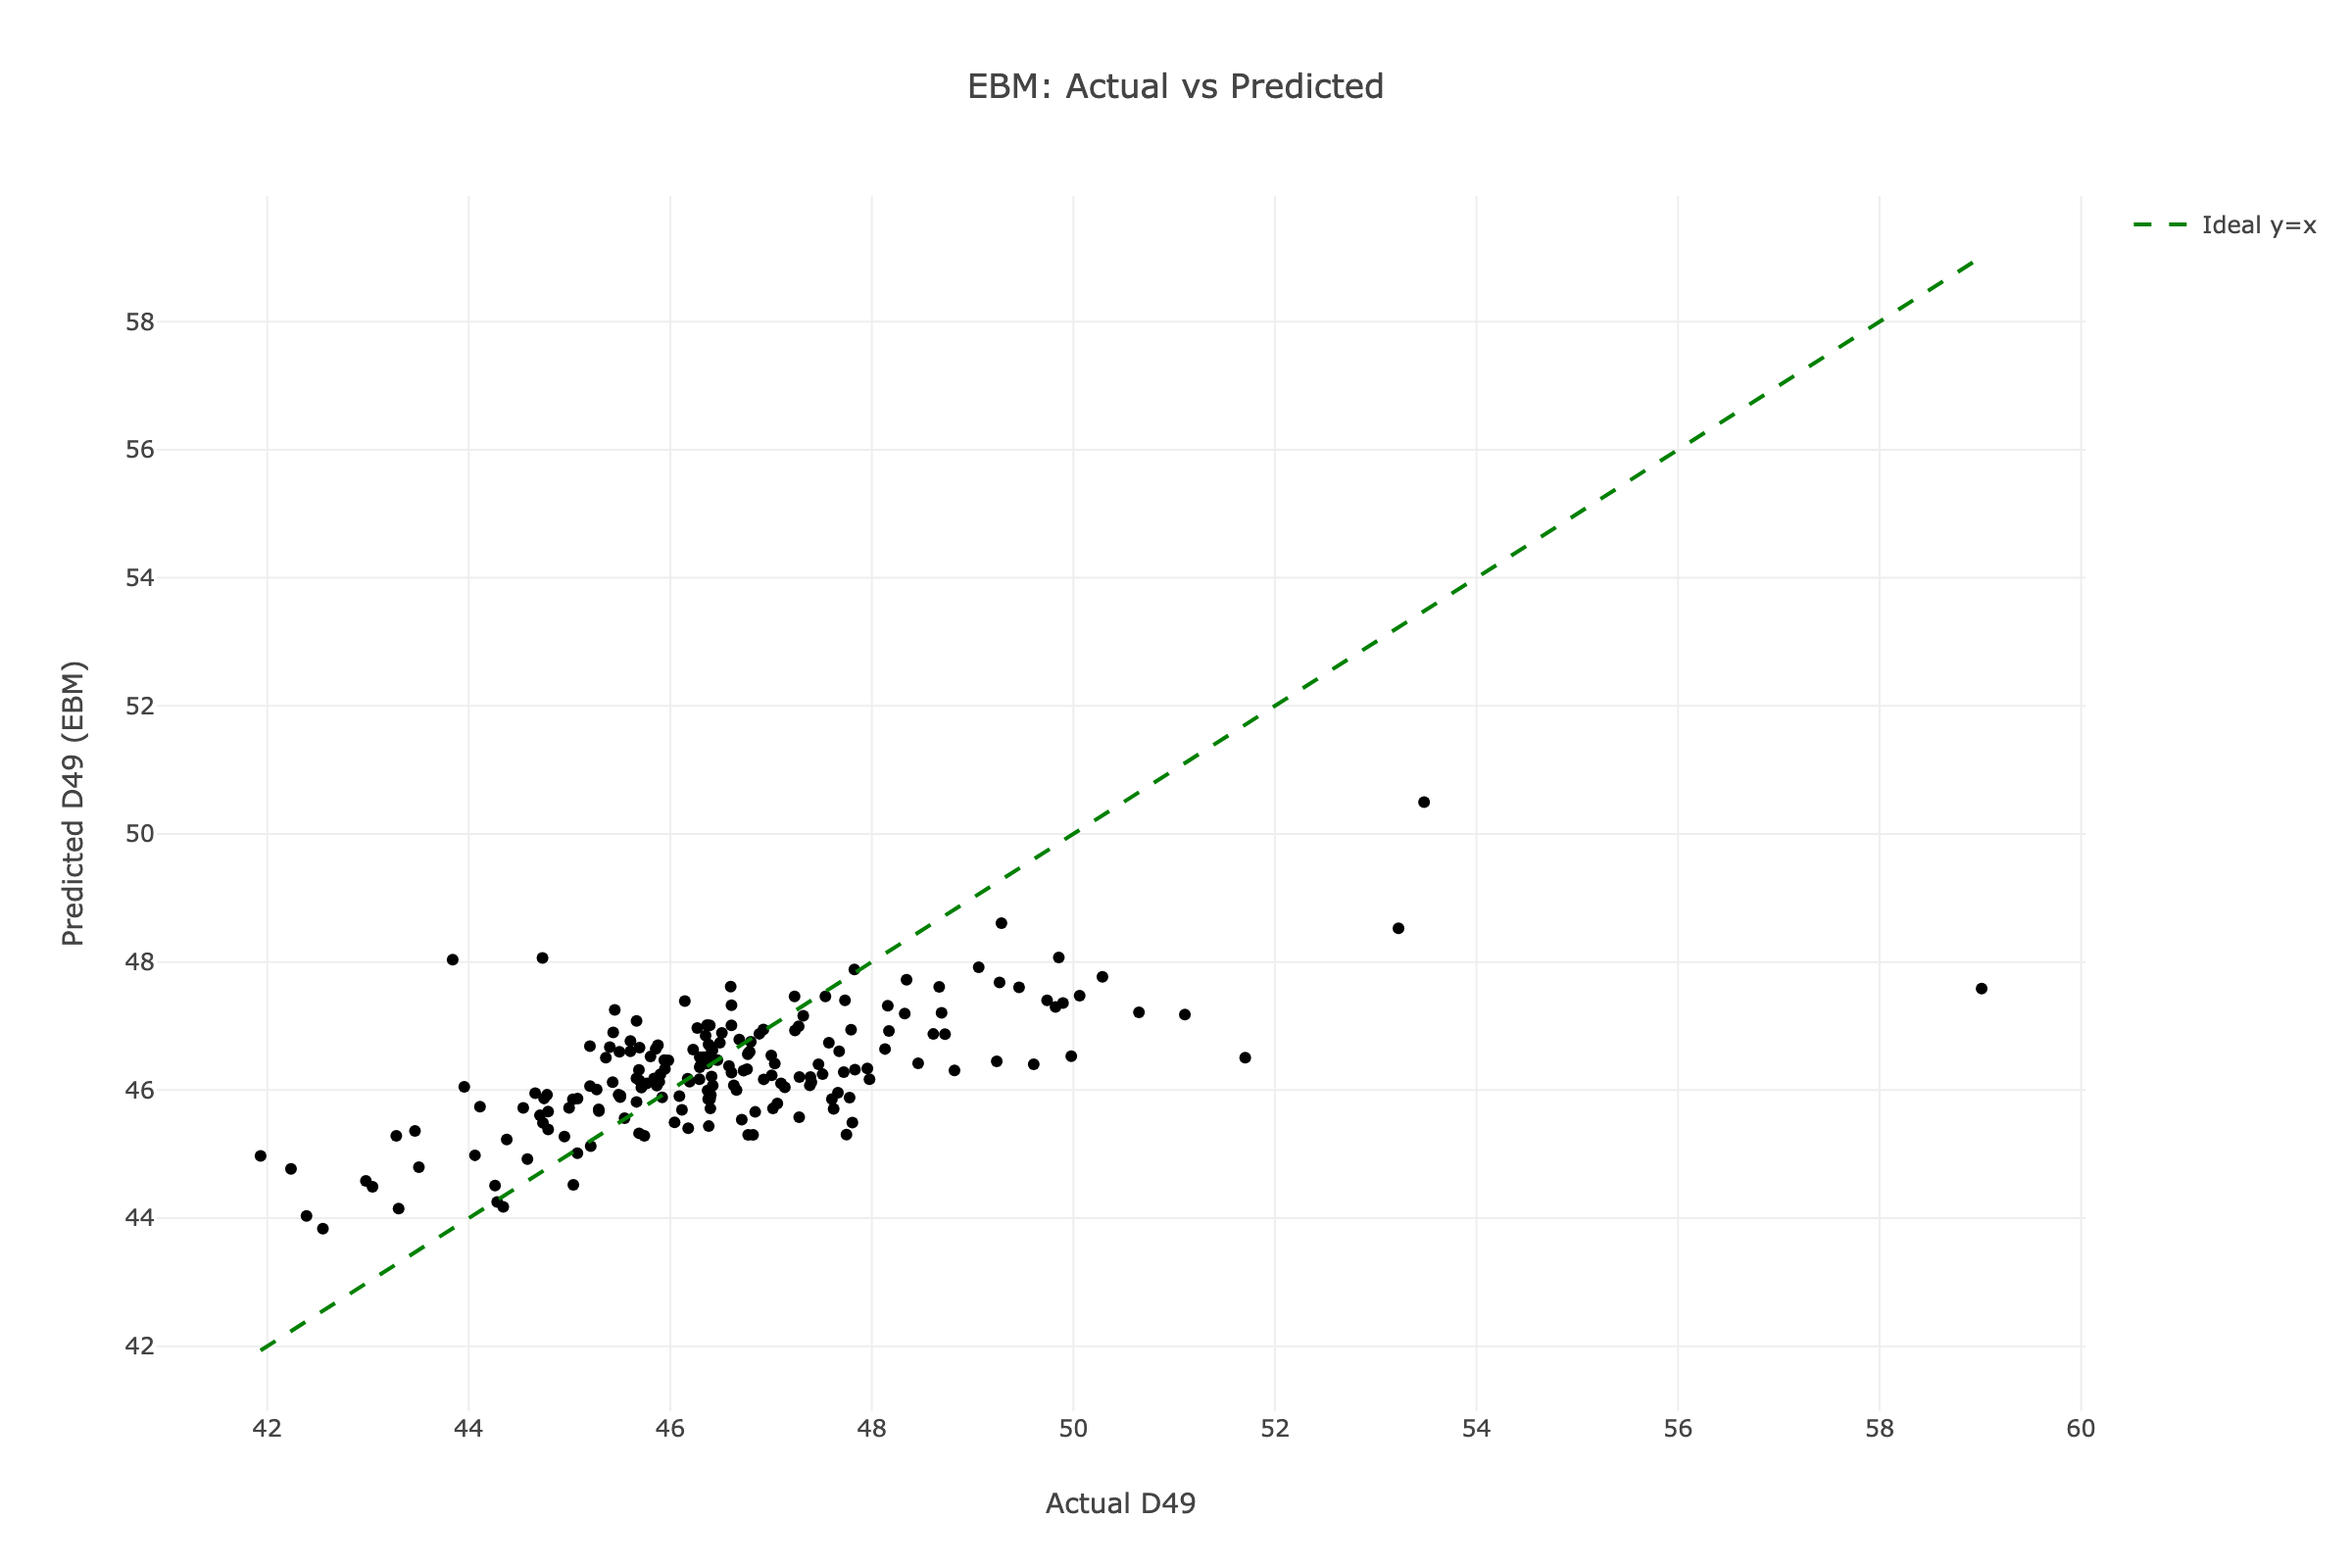
\includegraphics[width=\columnwidth]{images/fig_008_match_lasso_behavior_show_human_readable_name_next_to_encoded_feature_key.png}
    \caption{Predicció vs valor real (D49) del model EBM Fase 1 (sense interaccions). La línia discontínua representa la predicció perfecta ($y=x$).}
    \label{fig:ebm_phase1_actual_vs_pred}
\end{figure}

\subsubsection{Fase 2: Filtrat i reducció de dimensionalitat}
\label{subsubsec:fase2_filtrat_dimensionalitat}

Selecció de característiques basada en la importància apresa en Fase 1, reduint dimensionalitat i facilitant captura d'interaccions significatives.

\paragraph{Prova preliminar: Lasso $\rightarrow$ EBM (Top-10)}
Es va utilitzar el model Lasso com a filtre inicial, seleccionant les 10 característiques amb major importància per entrenar un model EBM.

El model EBM amb Top-10 Lasso va aconseguir MAE = 1.072, RMSE = 1.602, R² = 0.368.

La configuració final va seleccionar les \textbf{15 característiques més importants} (\texttt{top\_n = 15}), identificant el punt on la importància experimenta una caiguda significativa i mantenint variables amb major poder predictiu.

\subsubsection{Fase 3: Captura controlada d'interaccions}
\label{subsubsec:fase3_captura_interaccions}

La tercera i última fase entrena un model EBM sobre el conjunt reduït de característiques seleccionades en la Fase 2, activant la detecció automàtica d'interaccions. Aquesta configuració permet que el model identifiqui fins a 25 parells d'interaccions significatives (\texttt{interactions=25}) de manera automàtica.

Hiperparàmetres: \texttt{interactions=10} (detecció automàtica), \texttt{learning\_rate=0.05}, \texttt{max\_bins=256}, \texttt{max\_rounds=5000}, \texttt{min\_samples\_leaf=10}.

El model final va aconseguir un rendiment significativament millorat: MAE = 1.018, RMSE = 1.466 i R² = 0.470, demostrant l'efectivitat de la captura d'interaccions de manera controlada.

\begin{figure}[htbp]
    \centering
    \begin{subfigure}[b]{\columnwidth}
        \centering
        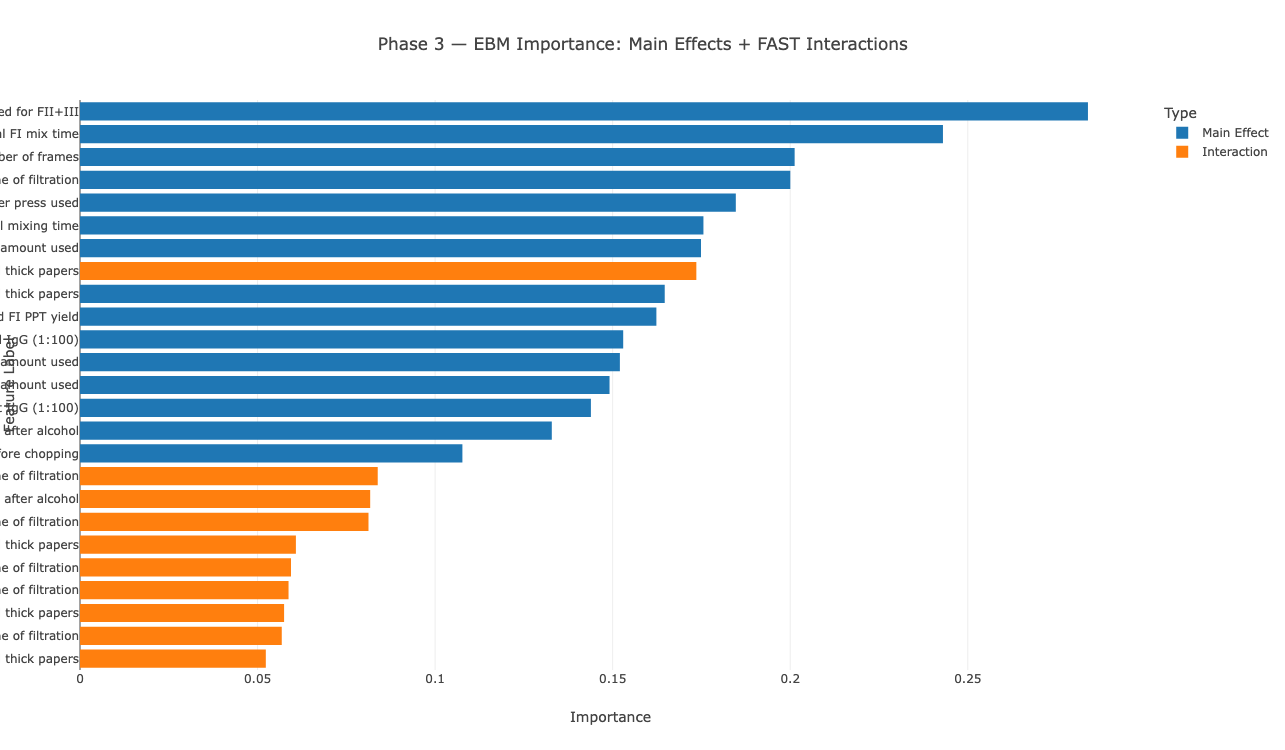
\includegraphics[width=0.95\columnwidth]{images/plot_importances.png}
        \caption{Efectes principals}
        \label{fig:ebm_phase3_main}
    \end{subfigure}
    \vspace{0.3em}
    \begin{subfigure}[b]{\columnwidth}
        \centering
        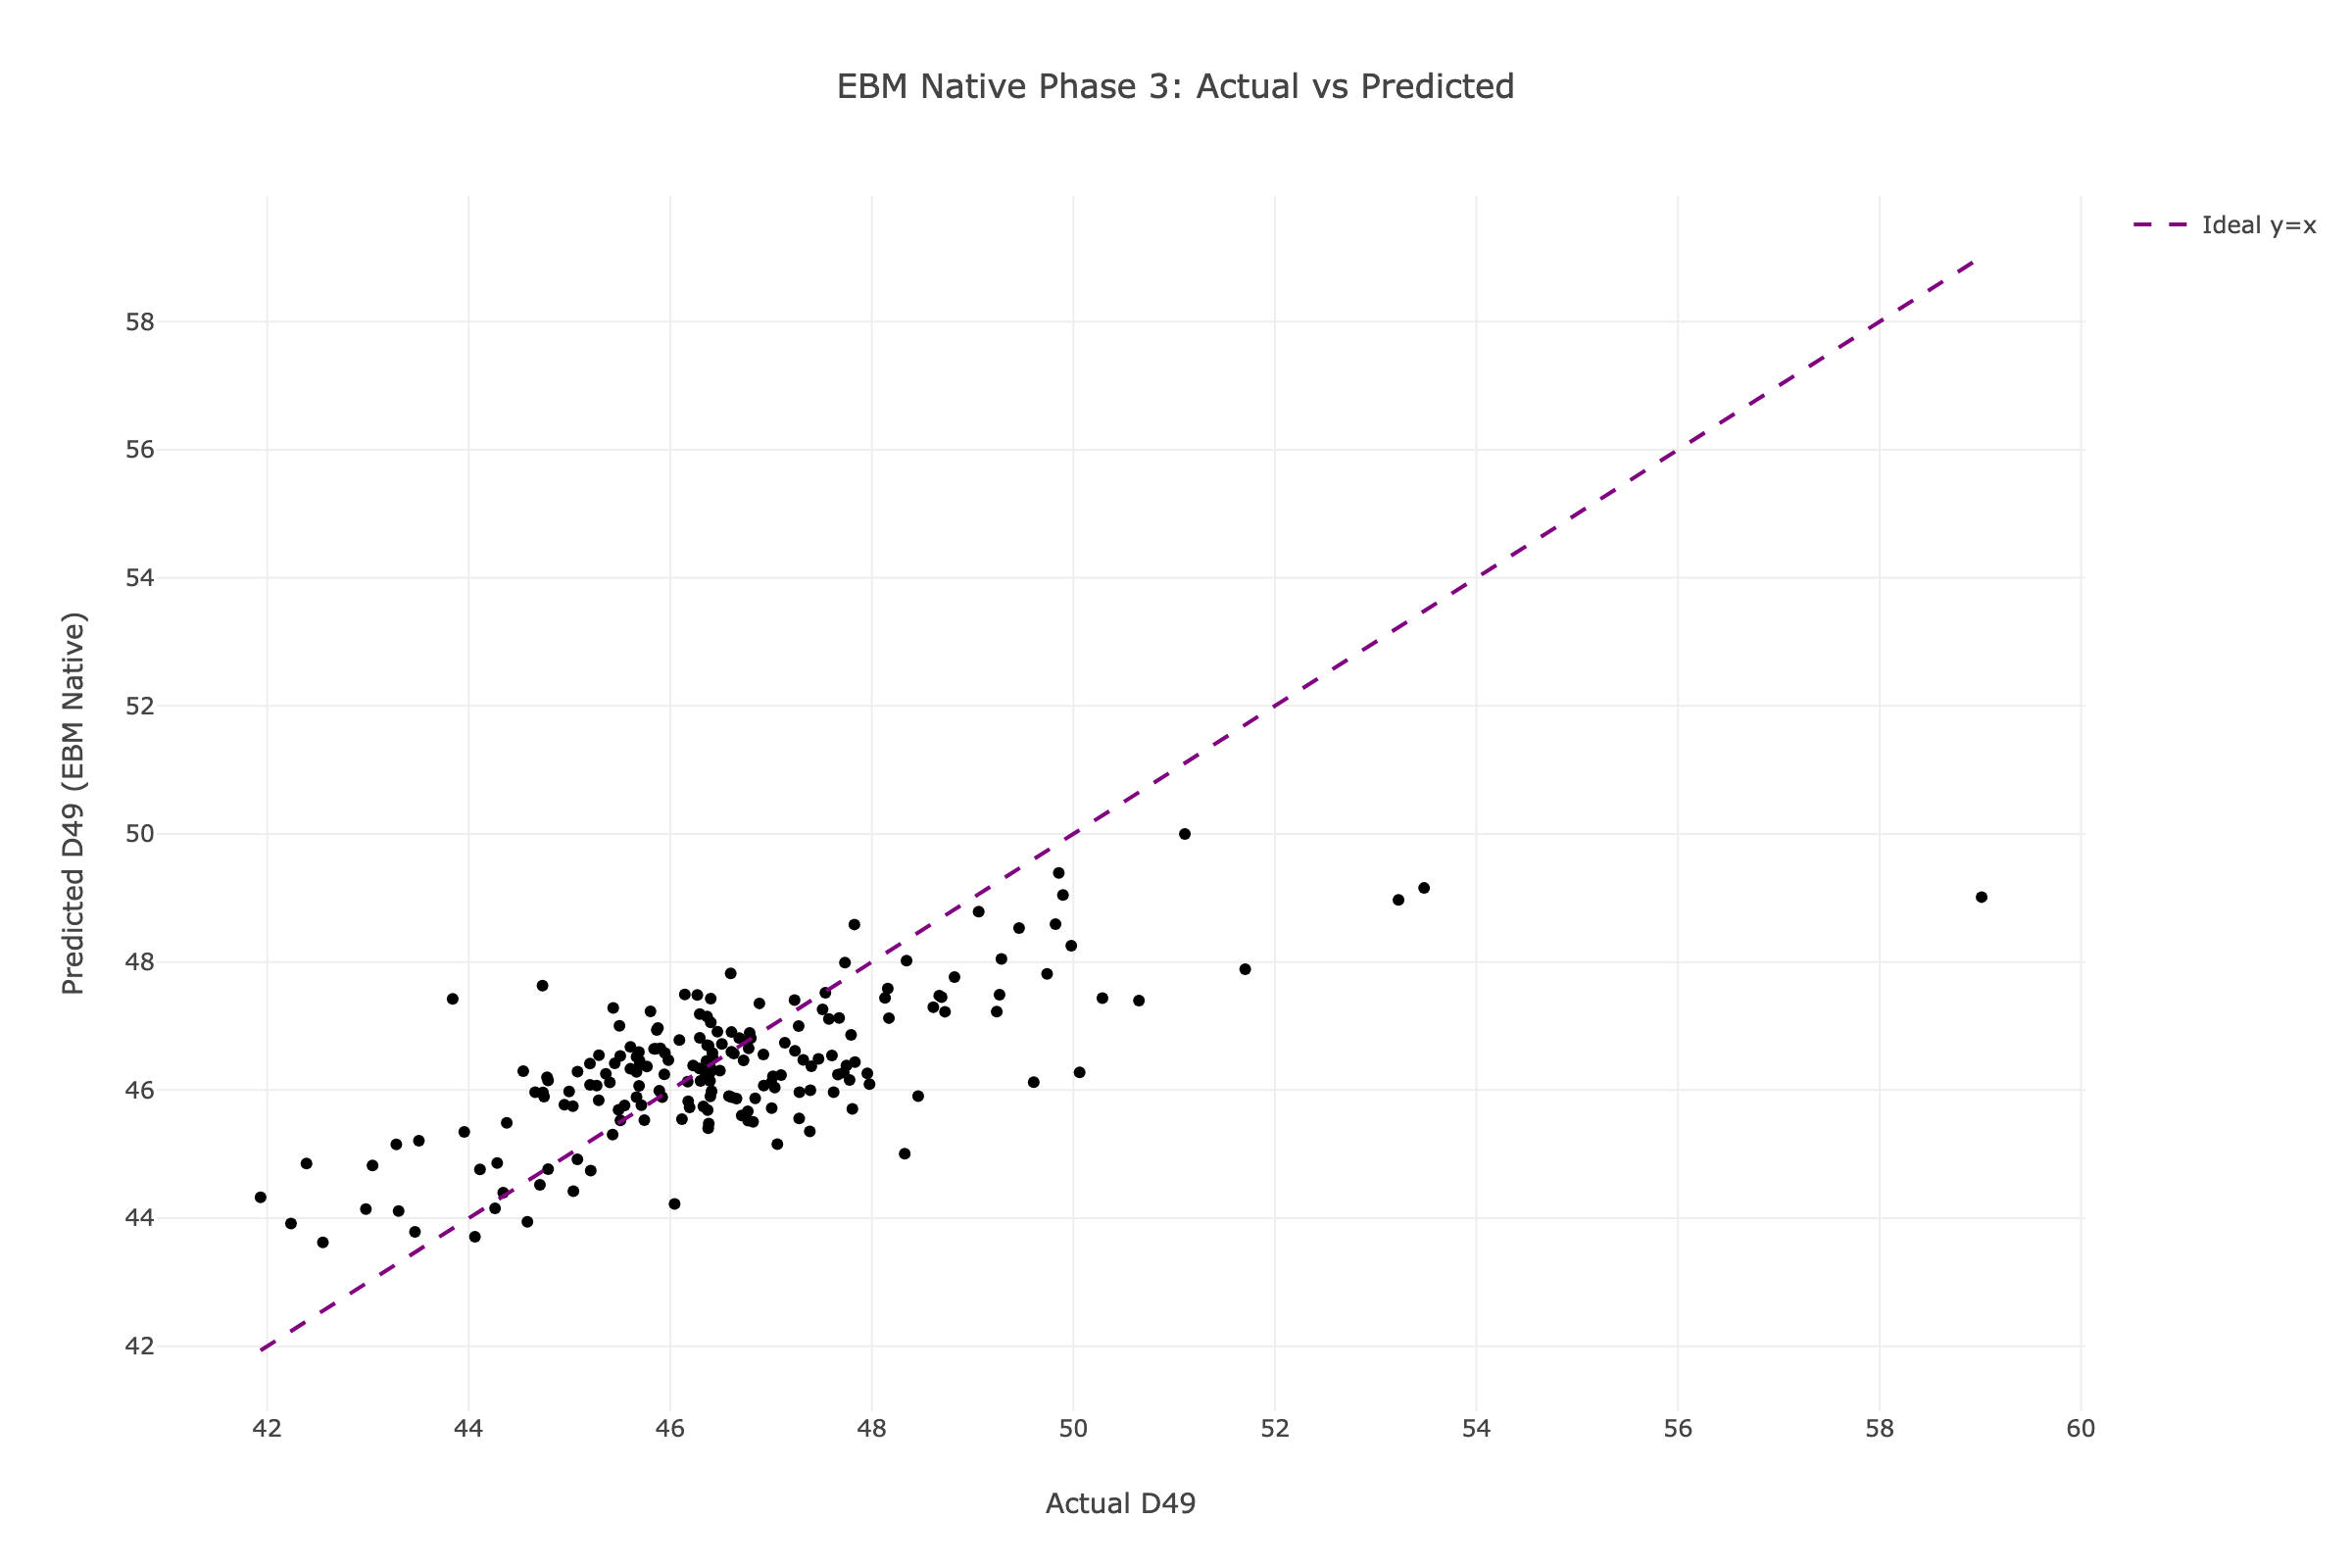
\includegraphics[width=0.95\columnwidth]{images/fig_014__extract_learned_terms_.png}
        \caption{Interaccions entre variables}
        \label{fig:ebm_phase3_interactions}
    \end{subfigure}
    \caption{Descomposició del model EBM Fase 3: (a) importància dels efectes principals de les 15 característiques seleccionades, (b) importància de les interaccions detectades automàticament pel model.}
    \label{fig:ebm_phase3_decomposition}
\end{figure}

La Figura \ref{fig:ebm_phase3_decomposition} mostra que el model captura efectes principals robustos i interaccions rellevants entre variables.

\subsubsection{Densitat de dades i control de complexitat}
\label{subsubsec:densitat_dades_control_complexitat}

La reducció de característiques (de 50+ variables a 15) redueix l'espai de cerca d'interaccions de O(n²) i garanteix suficients dades per estimar efectes principals i interaccions de manera fiable.

\subsection{Capa d'explicabilitat i Root Cause Analysis}
\label{subsec:capa_explicabilitat_rca}

Els models EBM proporcionen explicacions a diferents nivells. Tècniques utilitzades:

\begin{itemize}
    \item \textbf{Importància global de característiques:} Mesura de la contribució relativa de cada variable i interacció al rendiment general del model.
    \item \textbf{Shape functions:} Visualització de com cada característica afecta la predicció al llarg del seu rang de valors, capturant relacions no lineals.
    \item \textbf{Contribucions locals:} Descomposició de prediccions individuals per entendre quines variables i interaccions contribueixen a prediccions específiques.
    \item \textbf{Anàlisi d'interaccions:} Exploració de les relacions sinèrgiques entre parells de variables per identificar efectes combinats.
\end{itemize}

\subsection{Capa de validació i industrialització}
\label{subsec:capa_validacio_industrialitzacio}

Validació rigorosa del model i preparació per a implementació en entorns productius, garantint robustesa davant nous lots de producció.

\subsubsection{Validació d'hiperparàmetres i robustesa final}
\label{subsubsec:fase4_validacio_hiperparametres}

Es van explorar set configuracions diferents, variant bins (128, 256, 512), mostres per fulla (2, 5, 10), interaccions (15, 20, 25) i profunditat d'aprenentatge, identificant la configuració amb millor equilibri entre precisió, estabilitat i robustesa. Resultats detallats a la Secció~\ref{sec:resultats}.

\subsubsection{Preparació per a la industrialització}
\label{subsubsec:preparacio_industrialitzacio}

Aspectes clau: serialització i versionat del model (pickle/joblib amb metadades), pipeline de preprocessament documentat, sistema de monitoratge per detectar \emph{data/model drift}, integració amb sistemes MES via API REST, i documentació tècnica i operativa completa.

\subsubsection{Marc de validació GxP i posicionament del model}
\label{subsubsec:marc_validacio_gxp}

GAMP 5 \cite{gamp5} i la seva extensió per a IA/ML \cite{gamp_ai_ml} estableixen un cicle de validació basat en risc per a sistemes computaritzats en entorns GxP: especificació de requisits d'usuari (URS), avaluació de risc, qualificació d'instal·lació (IQ), operacional (OQ) i rendiment (PQ), control de canvis i monitoratge continu. La guia específica d'IA/ML \cite{gamp_ai_ml} adapta aquest cicle a models predictius, incorporant proves de rendiment estadístic, robustesa davant pertorbacions i detecció de drift com a elements d'OQ/PQ. L'Annex 11 d'EudraLex \cite{eudralex_annex11} reforça l'exigència de demostrar funcionament consistent i traçable.

El posicionament del model com a \emph{decision support} —no decisor automàtic— redueix la categoria de risc i l'esforç de validació requerit. La Taula~\ref{tab:gxp_positioning} resumeix l'estat actual respecte al marc GxP.

\begin{table}[htbp]
\centering
\caption{Posicionament del model respecte a requisits GxP}
\label{tab:gxp_positioning}
\footnotesize
\begin{tabular}{@{}p{0.42\columnwidth}p{0.50\columnwidth}@{}}
\toprule
\textbf{Cobert} & \textbf{Pendent} \\
\midrule
Interpretabilitat nativa (ALCOA+) & IQ/OQ/PQ formal \\
Pipeline documentat i versionat & Cobertura temporal ampliada \\
Monitoratge drift (PSI) & Protocol de change control \\
Ús previst delimitat (support) & Aprovació formal QA \\
Latència demostrada (OQ parcial) & Revalidació periòdica \\
\bottomrule
\end{tabular}
\end{table}

El drift detectat (PSI = 6.8 a D36) il·lustra empíricament la necessitat dels processos de revalidació que GAMP 5 exigeix. En conjunt, el treball construeix els fonaments tècnics —model interpretable, traçable i monitoritzat— sobre els quals es podria executar una validació GxP formal com a pas posterior.

